\documentclass[withoutpreface,bwprint]{cumcmthesis}

\usepackage[framemethod=TikZ]{mdframed}
\usepackage{tikz}
\usetikzlibrary{arrows.meta,calc}
\usepackage{url}
\usepackage{subcaption}
\usepackage{geometry}
\usepackage{ulem}
\usepackage{setspace}
\usepackage{array}
\usepackage{graphicx}
\usepackage{multirow}
\usepackage{hyperref}
\usepackage{amsmath}
\usepackage{longtable}
\usepackage{booktabs}
\graphicspath{{figures/}}

% 中文章节交叉引用（类文件仅定义了 figure/table/equation）
\crefformat{section}{#2第#1节#3}
\Crefformat{section}{#2第#1节#3}

\geometry{a4paper,left=25mm,right=25mm,top=25mm,bottom=25mm}
\title{基于红外干涉光谱的碳化硅与硅外延层厚度反演模型}

\begin{document}

\maketitle

% ======================================================================
% 摘要（模板：待定稿）
% ======================================================================
\begin{abstract}
碳化硅（SiC）与硅（Si）外延层的厚度是衡量半导体器件质量的关键指标，红外干涉光谱法凭借其非接触、无损、快速的优势成为主流测量手段。本文围绕外延层厚度反演问题，建立了从\textbf{双光束干涉}到\textbf{含吸收多光束（Airy/TMM）干涉}的逐级扩展模型，提出“修正波数域—多方案并行估计—双角度联合约束—多光束判定与修正”的总体求解框架，并对附件 1--4 给出可复现的厚度结果与不确定度区间。

\textbf{针对数据分析与预处理：} 本文将反射率分解为慢变基线、振幅包络与干涉条纹三部分，采用 Hampel 异常点剔除、Savitzky--Golay 轻度平滑、稳健多项式基线与包络归一化构造标准化条纹，并依据材料声子共振与色散特征划分有效拟合频段（SiC 取 $1500\sim4000\ \mathrm{cm^{-1}}$，Si 取 $550\sim3500\ \mathrm{cm^{-1}}$）。

\textbf{针对问题一：} 由斯涅尔定律定义修正波数 $x_\theta(\tilde\nu)=\tilde\nu\sqrt{n_1^2(\tilde\nu)-\sin^2\theta_0}$，同时吸收折射率色散与斜入射光程修正，建立双光束反射率模型 $R=A+B\cos(4\pi d x_\theta+\phi_0)+\varepsilon$，并给出相邻同类极值、峰级次稳健回归与 Hilbert 相位三种等价厚度反演关系。

\textbf{针对问题二、三：} （待定稿）综合 FFT 初值、峰级次回归、双角度联合拟合与 Hilbert 相位交叉验证，得到碳化硅外延层厚度约 $7.48\,\mu\mathrm m$；通过谐波、峰谷分离、可见度与 BIC 的联合判定确认硅数据存在显著多光束干涉，经基频隔离后得到硅外延层厚度约 $3.47\,\mu\mathrm m$。

\keywords{\textbf{红外干涉光谱\quad 修正波数\quad 双光束干涉\quad 多光束干涉\quad 厚度反演}}
\end{abstract}

% ======================================================================
% 1 问题重述（模板）
% ======================================================================
\section{问题重述}
\subsection{问题背景}
碳化硅、硅等半导体外延材料的性能与其外延层厚度密切相关。红外干涉法通过测量样品在中红外波段的反射率光谱，利用外延层上下界面反射光之间的干涉条纹反演厚度，是一种非接触、无损、高效的检测手段。

\subsection{问题提出}
题目提供四组红外反射光谱数据，第一列为波数（$\mathrm{cm^{-1}}$），第二列为反射率（\%）。其中附件 1、2 为同一 SiC 晶圆在 $10^\circ$、$15^\circ$ 入射角下的测量结果，附件 3、4 为同一 Si 晶圆在相同两个角度下的测量结果。需依次解决：

\begin{itemize}
	\item[(1)] 在只考虑外延层上下表面各一次反射（双光束）的条件下，建立红外反射光谱与外延层厚度的关系模型；
	\item[(2)] 基于该模型计算碳化硅外延层的厚度；
	\item[(3)] 分析多光束干涉可被观测的条件，判定硅数据（附件 3、4）中是否存在多光束干涉并据此求解硅外延层厚度；同时检验碳化硅数据是否受多光束干涉影响，若有则消除其影响给出修正结果。
\end{itemize}

% ======================================================================
% 2 问题分析（模板）
% ======================================================================
\section{问题分析}
外延层厚度反演的核心是把干涉条纹的周期与光学厚度联系起来。随着入射角与折射率色散的引入，简单的等波数间隔关系不再成立，需引入修正波数统一处理色散与斜入射；当界面反射较强、吸收较弱时，高阶内部反射不可忽略，双光束正弦模型应扩展为含吸收的多光束 Airy 模型。因此本文采用机理模型逐级扩展、多方案并行估计并相互验证的思路（详见后文各章）。

% ======================================================================
% 3 模型假设与符号说明（模板）
% ======================================================================
\section{模型假设与符号说明}
\subsection{模型假设}
\begin{itemize}
	\item[(1)] 空气、外延层与衬底均视为均匀、各向同性的平行分层介质；
	\item[(2)] 测量区域内外延层厚度近似恒定，上下界面近似平行；
	\item[(3)] 空气折射率取 $n_0=1$，外延层折射率 $n_1(\tilde\nu)$ 允许随波数变化；
	\item[(4)] 单个波数附近光源具有足够的相干长度；
	\item[(5)] 界面粗糙度、晶圆翘曲与仪器线形暂不进入主模型，仅在敏感性分析中考虑。
\end{itemize}

\subsection{符号说明}
本文常用符号如下，其余符号在使用处注明。
\begin{longtable}{cl}
	\toprule[1.5pt]
	符号 & \multicolumn{1}{c}{含义} \\
	\midrule[1pt]
	$\tilde\nu$ & 波数（$\mathrm{cm^{-1}}$）\\
	$R(\tilde\nu)$ & 反射率 \\
	$\theta_0$ & 外部入射角（$10^\circ$ 或 $15^\circ$）\\
	$\theta_1$ & 外延层内折射角 \\
	$n_0,n_1,n_2$ & 空气、外延层、衬底折射率 \\
	$x_\theta(\tilde\nu)$ & 修正波数 \\
	$d$ & 外延层厚度 \\
	$\Phi(\tilde\nu)$ & 双光束相位差 \\
	$A(\tilde\nu),B(\tilde\nu)$ & 慢变基线、条纹振幅包络 \\
	$\phi_0,\phi_r$ & 反射附加相位与起始级次 \\
	$\alpha(\tilde\nu)$ & 强度吸收系数 \\
	$\kappa(\tilde\nu)$ & 消光系数 \\
	$r_{01},r_{12}$ & 上、下界面 Fresnel 反射系数 \\
	$\eta$ & 相邻内部反射光复振幅比 \\
	$H_k$ & 第 $k$ 次谐波幅值 \\
	$V$ & 条纹可见度 \\
	\bottomrule[1.5pt]
\end{longtable}

% ======================================================================
% 4 数据分析与预处理
% ======================================================================
\section{数据分析与预处理}
红外干涉厚度反演依赖条纹的峰位与周期，改变峰位、抹平谷值或引入虚假周期的处理都可能给厚度带来系统偏差。为此，本文以“保留真实条纹、剔除与条纹无关的慢变背景及孤立异常”作为预处理的基本原则，并据此确定有效拟合频段。

\subsection{数据特征与有效频段选取}

\subsubsection{数据映射与质量检查}
四组附件均为等波数近似采样的反射率光谱，原始各含 $7469$ 行，其中首行均为反射率异常偏零的无效点，按统一规则删除后各余 $7468$ 个有效点。四组数据的材料、入射角与量程如\cref{tab:data_map} 所示。

\begin{table}[!htbp]
	\centering
	\caption{附件数据映射与质量检查}\label{tab:data_map}
	\begin{tabular}{ccccccc}
		\toprule
		附件 & 材料 & 入射角 & 有效点数 & 波数范围/$\mathrm{cm^{-1}}$ & 反射率范围/\% & 超 100\% 比例 \\
		\midrule
		附件 1 & SiC & $10^\circ$ & 7468 & 400.16--4000.12 & 0.636--95.385 & 0 \\
		附件 2 & SiC & $15^\circ$ & 7468 & 400.16--4000.12 & 0.977--102.739 & 3.508\% \\
		附件 3 & Si  & $10^\circ$ & 7468 & 400.16--4000.12 & 0.134--79.802 & 0 \\
		附件 4 & Si  & $15^\circ$ & 7468 & 400.16--4000.12 & 0.349--91.489 & 0 \\
		\bottomrule
	\end{tabular}
\end{table}

数据检查得到三点关键结论：

\begin{itemize}
	\item[(1)] \textbf{采样间隔}。四组数据波数间隔的中位数约为 $0.482\ \mathrm{cm^{-1}}$，采样密度足够刻画中红外条纹，不构成分辨率瓶颈；但间隔并非严格等距，故所有频域运算前需将信号插值到等间距网格。
	\item[(2)] \textbf{附件 2 的超量程反射率}。附件 2 约有 $3.508\%$ 的反射率超过 $100\%$，这源于测量标定或归一化偏差。若直接硬截断，会削平条纹峰并改变峰位。本文将其写为标定关系
	\begin{equation}
		R_{\mathrm{obs}}=g\,R_{\mathrm{model}}+c+\varepsilon
		\label{eq:calib}
	\end{equation}
	通过增益 $g$、偏置 $c$ 以及后续基线—包络归一化吸收该偏差，而不做截断。
	\item[(3)] \textbf{孤立异常点}。除首点外，各组仍存在少量孤立跳变点，需以稳健方法逐点识别（见\cref{sec:preprocess}）。
\end{itemize}

\subsubsection{有效频段选取}
选取有效频段的依据是：拟合区间应落在材料透明、折射率随波数缓变的窗口内，避开强声子共振与强色散区，从而保证实折射率双光束模型的适用性。

对 SiC，其横光学（TO）声子约在 $797.7\ \mathrm{cm^{-1}}$、纵光学（LO）声子约在 $992.1\ \mathrm{cm^{-1}}$，$800\sim1100\ \mathrm{cm^{-1}}$ 为剩余射线强反射带，折射率剧烈色散甚至出现负介电区，简单模型失效。因此本文取

\begin{equation}
	\text{SiC 主拟合频段：}\quad 1500\sim4000\ \mathrm{cm^{-1}}
\end{equation}

并以 $1100\sim1500\ \mathrm{cm^{-1}}$ 作为辅助验证区间，$800\sim1100\ \mathrm{cm^{-1}}$ 仅在需要复介电函数时使用。对 Si，中红外无强声子吸收，透明窗口宽，取

\begin{equation}
	\text{Si 主拟合频段：}\quad 550\sim3500\ \mathrm{cm^{-1}}
\end{equation}

\cref{fig:raw_overview} 给出四组原始光谱的总体形态，与上述频段选取一致：SiC 在 $800\sim1100\ \mathrm{cm^{-1}}$ 的剩余射线带（红色阴影）反射率接近饱和且不含有效条纹，主频段（绿色）内则呈现清晰的小幅正弦条纹；Si 无强声子吸收，透明窗口内条纹幅度较大、周期规则，可在较宽频段内反演。

\begin{figure}[!htbp]
	\centering
	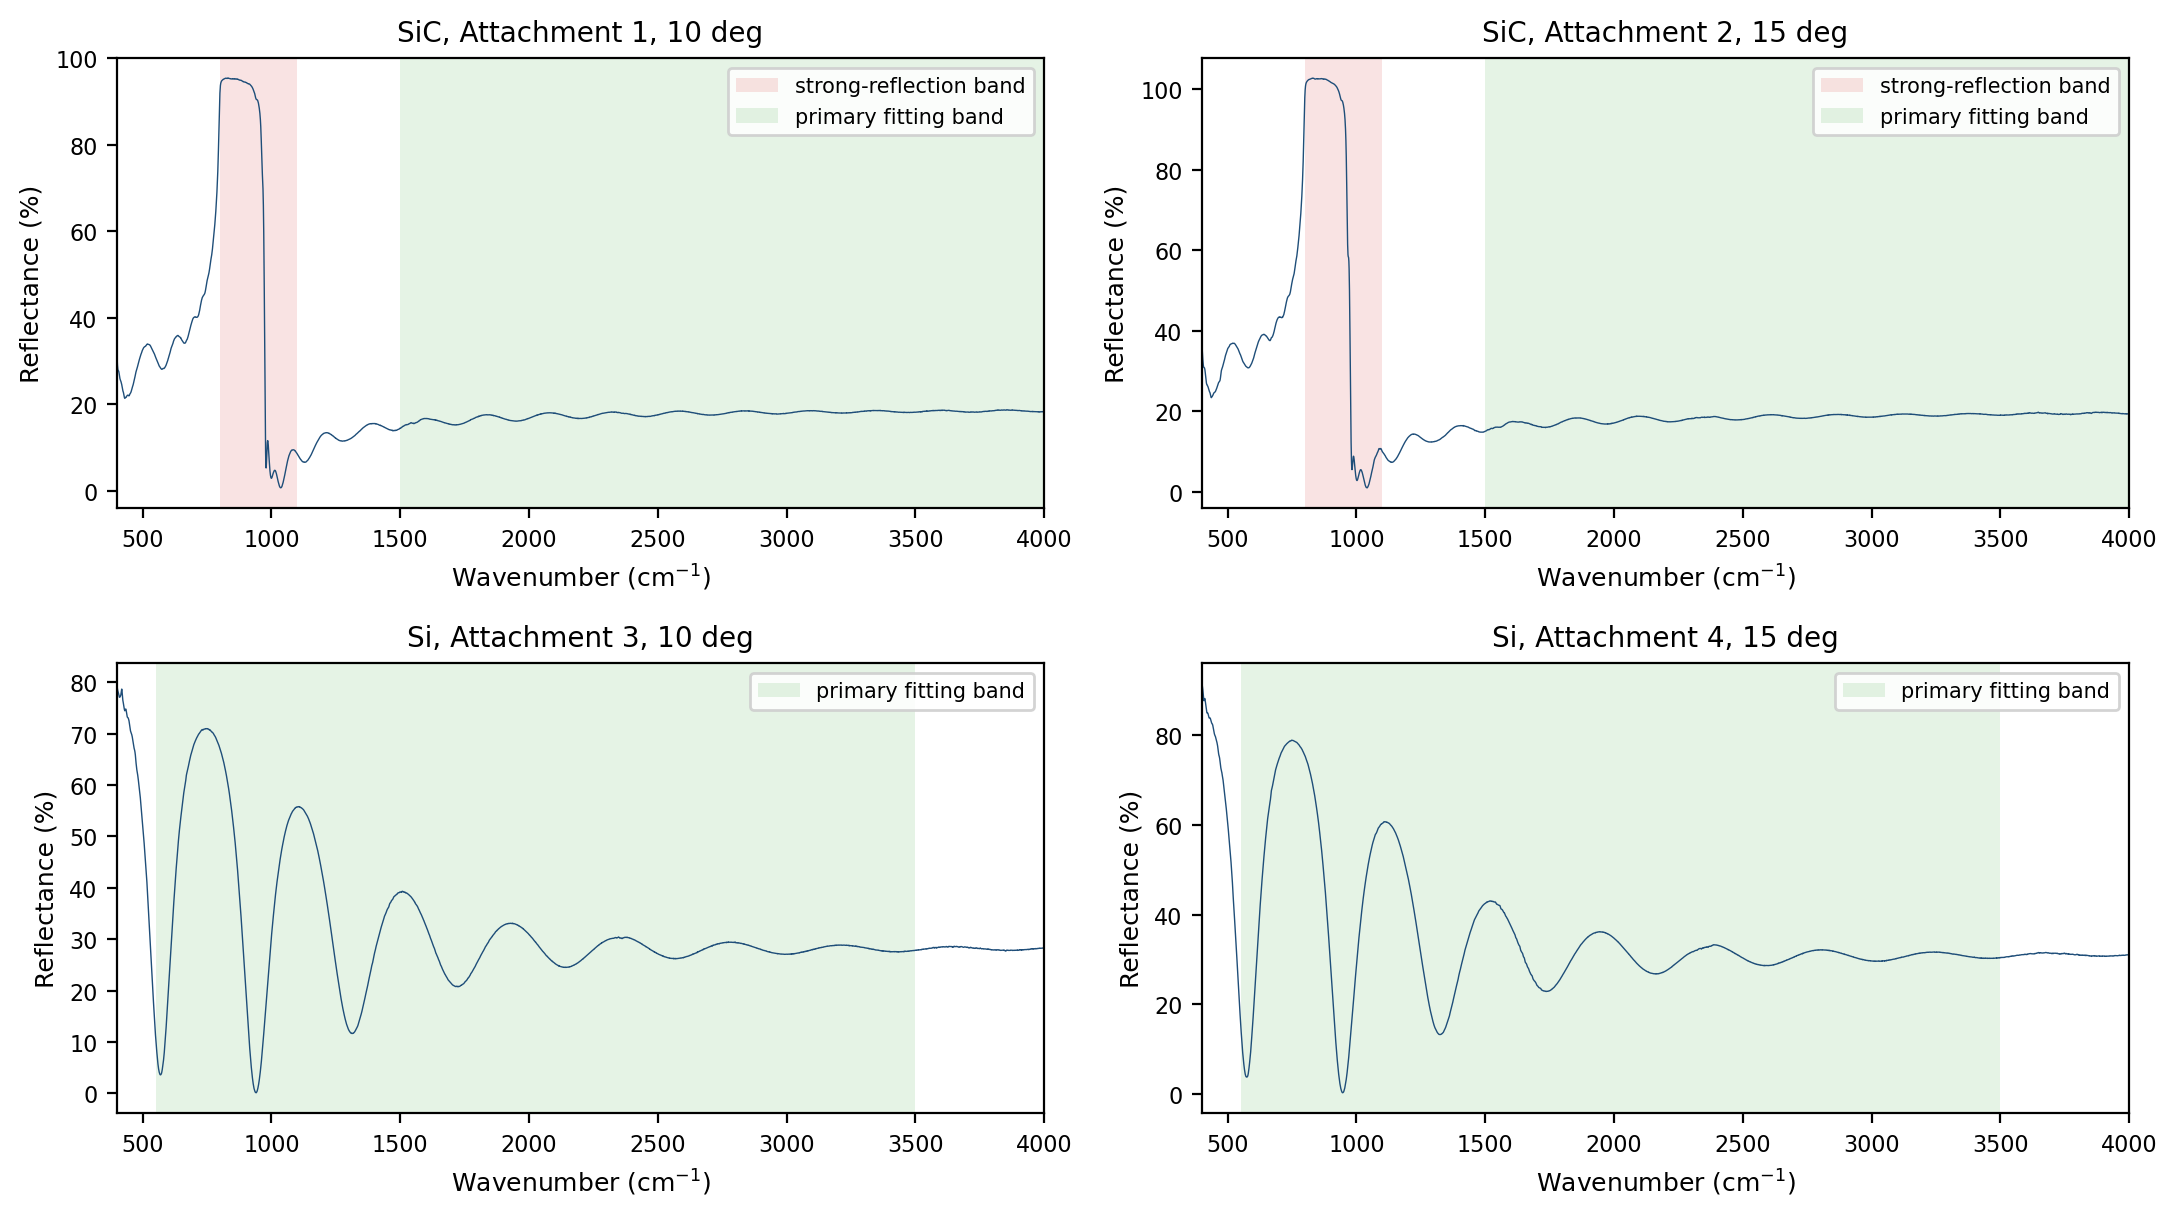
\includegraphics[width=\textwidth]{raw_overview}
	\caption{附件 1--4 原始反射光谱总体形态与频段划分（红色：SiC 强反射带；绿色：主拟合频段）}\label{fig:raw_overview}
\end{figure}

频段选取的合理性可由分频段稳定性检验进一步说明。将主频段与若干相邻子区间分别独立反演，结果如\cref{tab:band} 所示。主频段内四种方法的中位厚度相对共识值的偏离最小（SiC 约 $0.8\%$，Si 约 $3\%\sim4\%$）；而在低波数验证区（如 SiC 的 $1100\sim1500\ \mathrm{cm^{-1}}$、Si 的 $550\sim1500\ \mathrm{cm^{-1}}$），因条纹数偏少且色散增强，FFT 等方法出现明显漂移。这一对比表明将主频段避开低波数强色散区是必要的。

\begin{table}[!htbp]
	\centering
	\caption{分频段厚度稳定性（峰级次法结果，单位 $\mu\mathrm m$）}\label{tab:band}
	\begin{tabular}{cccccc}
		\toprule
		材料 & 频段/$\mathrm{cm^{-1}}$ & $10^\circ$ 峰级次 & $15^\circ$ 峰级次 & 相对共识偏离 \\
		\midrule
		SiC & 主频段 $1500\sim4000$ & 7.489 & 7.463 & $-0.82\%$ \\
		SiC & 验证区 $1800\sim2800$ & 7.376 & 7.346 & $+6.3\%\sim8.9\%$ \\
		SiC & 验证区 $2800\sim4000$ & 7.747 & 7.738 & $+3.1\%\sim5.8\%$ \\
		Si  & 主频段 $550\sim3500$  & 3.477 & 3.467 & $+3.3\%\sim4.1\%$ \\
		Si  & 验证区 $1500\sim2500$ & --    & --    & $-5.7\%\sim-10.8\%$ \\
		\bottomrule
	\end{tabular}
\end{table}

\subsection{光谱预处理与标准化}\label{sec:preprocess}
本文将测得反射率分解为三个尺度成分：

\begin{equation}
	R(\tilde\nu)=\underbrace{A(\tilde\nu)}_{\text{慢变基线}}+\underbrace{B(\tilde\nu)}_{\text{振幅包络}}\,y(\tilde\nu)+\varepsilon(\tilde\nu)
	\label{eq:decomp}
\end{equation}

其中 $A$ 描述平均反射率、仪器背景与慢变吸收，$B$ 描述条纹振幅随波数的缓变，$y$ 为归一化条纹，$\varepsilon$ 为噪声。预处理即依次估计并剥离 $A$、$B$，得到便于峰检测、FFT 与 Hilbert 变换的标准化条纹。处理链共四步。

\paragraph{（1）异常点剔除。}
采用 Hampel 方法：以窗口长度 $7$ 计算局部中位数与稳健标准差（MAD），将偏离超过 $3.5$ 倍稳健标准差的点判为孤立异常并以局部中位数替换。该方法只修正孤立跳变，不改变连续条纹。附件 1--4 分别检出 $13$、$21$、$4$、$5$ 个异常点。

\paragraph{（2）轻度平滑。}
采用 Savitzky--Golay 滤波\upcite{savitzky1964smoothing}，以窗口 $21$、多项式阶数 $3$ 在最小二乘意义下局部拟合，抑制高频噪声同时保留峰形。窗口不能过大，否则会造成峰位偏移、尖锐谷值被抹平、相邻条纹合并以及多光束高次谐波被误删。本文在 $11,21,31,41$ 等窗口中以厚度结果稳定性择优，最终取 $21$。

\paragraph{（3）基线与包络校正。}
以稳健迭代多项式（阶数 $3$、迭代 $6$ 次）估计慢变基线 $\widehat A(\tilde\nu)$\upcite{eilers2003baseline}；再以窗口 $301$、阶数 $2$ 的多项式估计振幅包络 $\widehat B(\tilde\nu)$，并设包络下限为量程的 $8\%$ 以防除零。

\paragraph{（4）标准化条纹。}
由\cref{eq:decomp} 构造标准化条纹

\begin{equation}
	z(\tilde\nu)=\frac{R(\tilde\nu)-\widehat A(\tilde\nu)}{\widehat B(\tilde\nu)}
	\label{eq:zfringe}
\end{equation}

其理想形态为零均值、单位振幅的余弦条纹。峰值检测、FFT 与 Hilbert 变换均在 $z(\tilde\nu)$ 上进行，从而使结果对慢变背景与振幅漂移不敏感。\cref{fig:preprocess} 给出 SiC（附件 1）与 Si（附件 3）主频段的预处理效果，可见基线—包络剥离后条纹被有效标准化。

\begin{figure}[!htbp]
	\centering
	\begin{subfigure}[b]{0.48\textwidth}
		\centering
		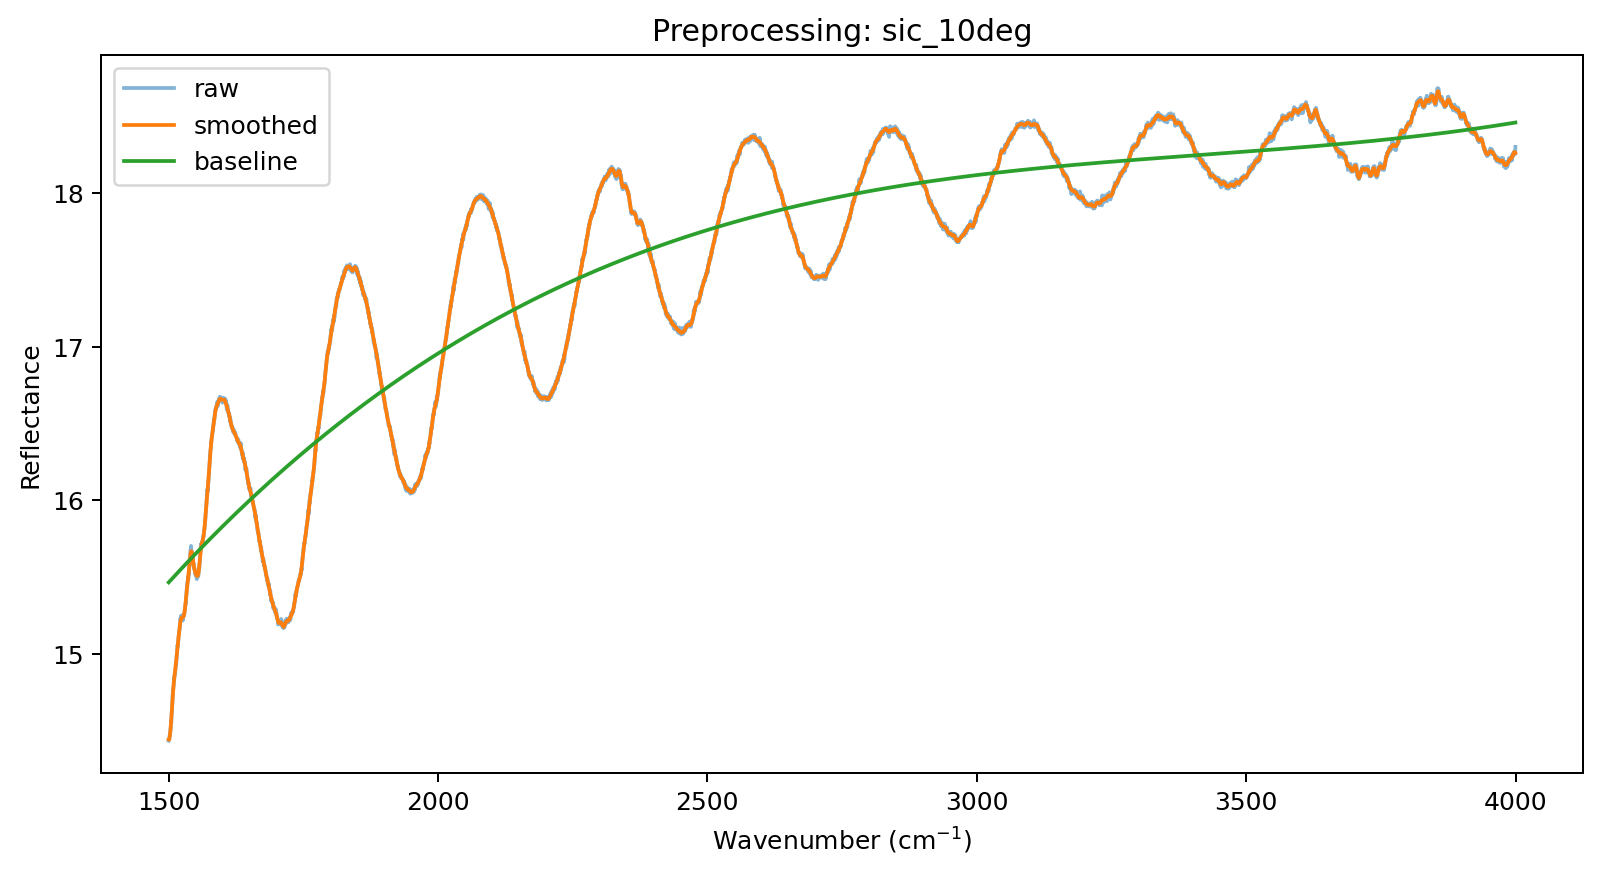
\includegraphics[width=\textwidth]{preprocess_sic_10deg}
		\caption{SiC，附件 1，$10^\circ$}
	\end{subfigure}
	\hfill
	\begin{subfigure}[b]{0.48\textwidth}
		\centering
		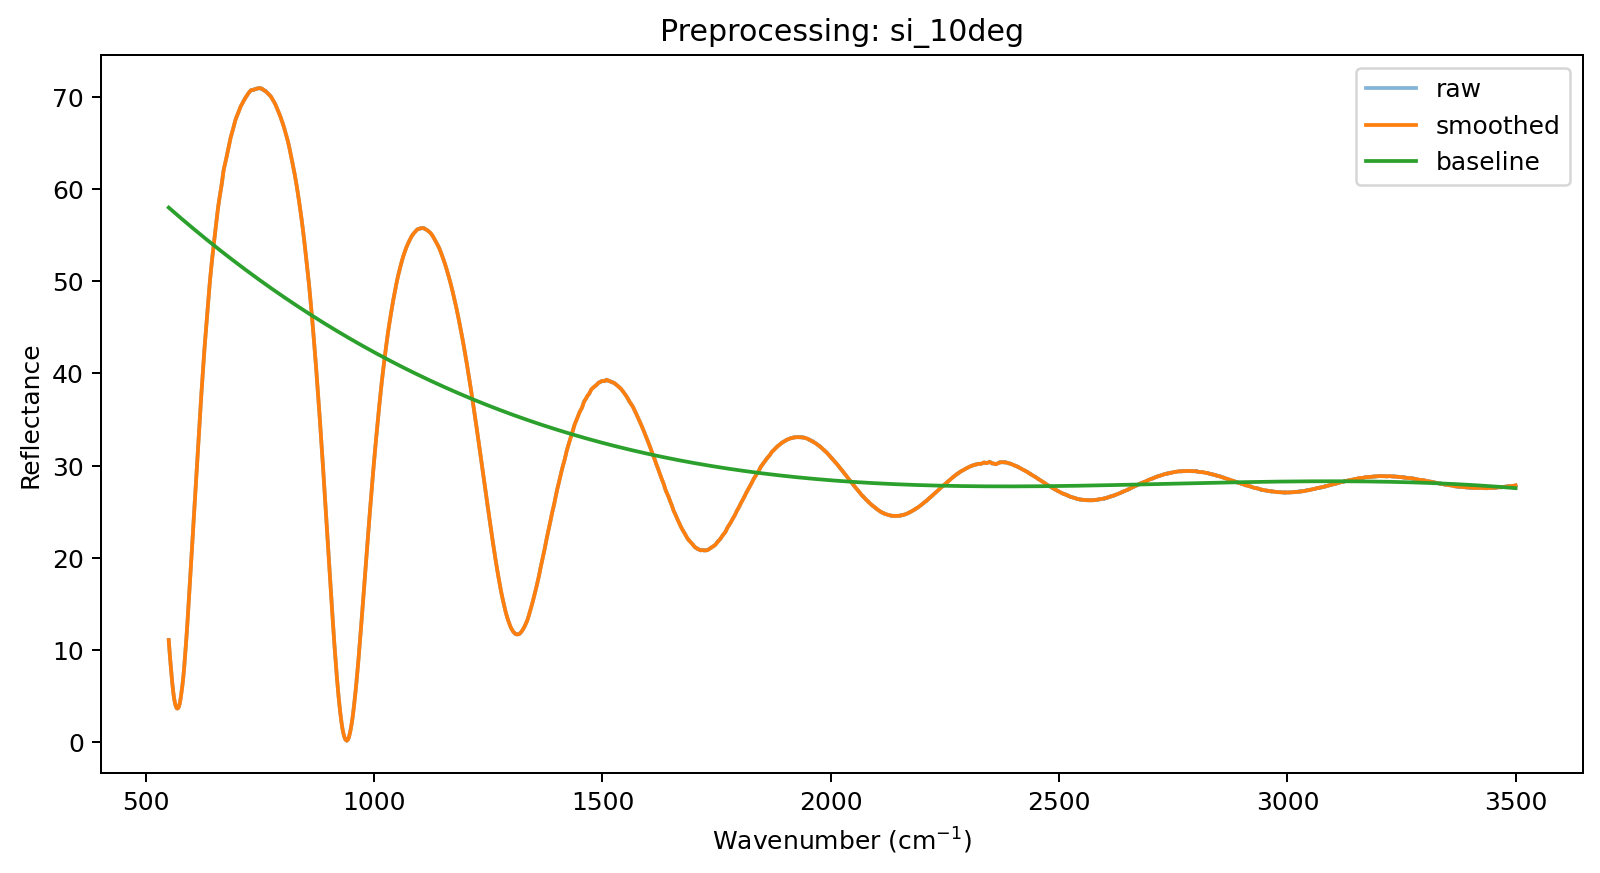
\includegraphics[width=\textwidth]{preprocess_si_10deg}
		\caption{Si，附件 3，$10^\circ$}
	\end{subfigure}
	\caption{主频段光谱预处理与标准化条纹}\label{fig:preprocess}
\end{figure}

经过上述四步处理，预处理在剔除异常、抑制噪声的同时保留了条纹的周期与峰位信息，为后续各章的厚度反演提供了统一、稳健的输入。

% ======================================================================
% 5 问题一：一次反射条件下的双光束干涉模型
% ======================================================================
\section{问题一：一次反射条件下的双光束干涉模型}
问题一在只考虑两束反射光的条件下建立红外反射光谱与外延层厚度之间的关系：第一束光在空气—外延层表面直接反射，第二束光进入外延层并在外延层—衬底界面反射一次后返回，两束光叠加形成干涉条纹。该模型是问题二、三全部厚度反演算法的理论基础。其几何关系如\cref{fig:twobeam} 所示。

\begin{figure}[!htbp]
	\centering
	\begin{tikzpicture}[scale=1.0,>=Stealth]
		% layers
		\fill[gray!8]  (0,2) rectangle (8,3.2);      % air label region
		\fill[cyan!12] (0,0) rectangle (8,2);        % epilayer
		\fill[gray!30] (0,-1.1) rectangle (8,0);     % substrate
		\draw[thick] (0,2)--(8,2);                    % top interface
		\draw[thick] (0,0)--(8,0);                    % bottom interface
		% labels of media
		\node at (7.0,2.65) {空气 $n_0$};
		\node at (7.0,1.0)  {外延层 $n_1(\tilde\nu)$};
		\node at (7.0,-0.55){衬底 $n_2(\tilde\nu)$};
		% incident ray
		\draw[->,thick,blue] (1.2,3.1)--(3.0,2.0);
		% first reflected (surface)
		\draw[->,thick,blue] (3.0,2.0)--(4.8,3.1);
		% refracted into layer
		\draw[thick,blue] (3.0,2.0)--(4.2,0.0);
		% reflect at bottom
		\draw[thick,blue] (4.2,0.0)--(5.4,2.0);
		% second emerging beam
		\draw[->,thick,blue] (5.4,2.0)--(7.2,3.1);
		% normal at top
		\draw[dashed] (3.0,2.0)--(3.0,3.3);
		\draw[dashed] (5.4,2.0)--(5.4,3.3);
		% angles
		\node at (2.75,2.55) {$\theta_0$};
		\node at (3.42,1.35) {$\theta_1$};
		% thickness marker
		\draw[<->] (0.35,0.0)--(0.35,2.0);
		\node[left] at (0.35,1.0) {$d$};
		% beam labels
		\node[blue] at (4.9,3.35) {束1};
		\node[blue] at (7.25,3.35) {束2};
	\end{tikzpicture}
	\caption{双光束干涉几何示意：表面直接反射光（束1）与一次内部反射光（束2）}\label{fig:twobeam}
\end{figure}

\subsection{光程差与干涉相位}
设外部入射角为 $\theta_0$，外延层内折射角为 $\theta_1$。由斯涅尔定律，

\begin{equation}
	n_0\sin\theta_0=n_1(\tilde\nu)\sin\theta_1
	\label{eq:snell}
\end{equation}

取 $n_0=1$，则

\begin{equation}
	n_1(\tilde\nu)\cos\theta_1=\sqrt{n_1^2(\tilde\nu)-\sin^2\theta_0}
	\label{eq:cos1}
\end{equation}

第二束光在外延层内完成一次往返，其相对第一束光的光学程差为

\begin{equation}
	\operatorname{OPD}=2d\,n_1(\tilde\nu)\cos\theta_1
	\label{eq:opd}
\end{equation}

对波数 $\tilde\nu=1/\lambda$，传播相位差为

\begin{equation}
	\Phi_p(\tilde\nu)=2\pi\tilde\nu\operatorname{OPD}=4\pi d\,\tilde\nu\,n_1(\tilde\nu)\cos\theta_1
	\label{eq:phip}
\end{equation}

计入两界面 Fresnel 反射引入的附加相位 $\phi_r$，双光束总相位差为

\begin{equation}
	\Phi(\tilde\nu)=4\pi d\,x_\theta(\tilde\nu)+\phi_r
	\label{eq:Phi}
\end{equation}

其中 $x_\theta$ 为下节定义的修正波数。

\subsection{修正波数与双光束反射率模型}
若直接以原始波数 $\tilde\nu$ 作横轴，则由于 $n_1(\tilde\nu)\cos\theta_1$ 随波数变化，条纹并非严格等间隔，普通 FFT 与峰间距法会产生系统偏差。为此定义\textbf{修正波数}

\begin{equation}
	x_\theta(\tilde\nu)=\tilde\nu\sqrt{n_1^2(\tilde\nu)-\sin^2\theta_0}
	\label{eq:xtheta}
\end{equation}

将\cref{eq:cos1} 代入\cref{eq:phip}，传播相位差化为 $\Phi_p=4\pi d\,\tilde\nu\,n_1\cos\theta_1=4\pi d\,x_\theta$，即修正波数把折射率色散与斜入射光程修正一并并入相位的线性项。因此，此后的 FFT、峰级次回归、Hilbert 相位与联合拟合均在 $x_\theta$ 域进行，而非直接在原始波数域进行。

设两束反射光的慢变强度分别为 $I_1(\tilde\nu)$、$I_2(\tilde\nu)$，则

\begin{equation}
	R(\tilde\nu)=I_1+I_2+2\sqrt{I_1 I_2}\cos\Phi(\tilde\nu)+\varepsilon(\tilde\nu)
	\label{eq:Rraw}
\end{equation}

将慢变部分合并为基线 $A(\tilde\nu)=I_1+I_2$ 与振幅包络 $B(\tilde\nu)=2\sqrt{I_1 I_2}$，即得用于计算的双光束反射率模型

\begin{equation}
	R(\tilde\nu)=A(\tilde\nu)+B(\tilde\nu)\cos\!\left[4\pi d\,x_\theta(\tilde\nu)+\phi_0\right]+\varepsilon(\tilde\nu)
	\label{eq:twobeam}
\end{equation}

其中 $\phi_0$ 吸收未知反射相位与起始级次。该模型与\cref{eq:decomp} 的预处理分解相互对应：$A$、$B$ 即预处理所剥离的基线与包络，故标准化条纹满足 $z(\tilde\nu)\approx\cos[4\pi d x_\theta+\phi_0]$。

同一材料的两个附件取自同一块晶圆，故两个角度共享同一厚度 $d$ 与折射率 $n_1(\tilde\nu)$，而各自具有独立的背景、包络与相位：

\begin{equation}
	R_k(\tilde\nu)=A_k(\tilde\nu)+B_k(\tilde\nu)\cos\!\left[4\pi d\,x_k(\tilde\nu)+\phi_k\right]+\varepsilon_k,\quad k\in\{10^\circ,15^\circ\}
	\label{eq:shared}
\end{equation}

由于两个角度的相位、背景与振幅各不相同，其反射率不能直接平均；合理的做法是共享厚度、分别拟合角度特有参数，这也是后续双角度一致性检验的基础。

\subsection{厚度反演关系}
由模型\cref{eq:twobeam} 出发，可导出三种相互独立而互补的厚度反演关系。在修正波数横轴上，相位每增加 $2\pi$ 对应一个条纹周期。

\paragraph{（1）相邻同类极值法。}
相邻峰—峰或谷—谷之间相位恰增加 $2\pi$：

\begin{equation}
	4\pi d\,(x_{m+1}-x_m)=2\pi\;\Longrightarrow\;d=\frac{1}{2(x_{m+1}-x_m)}=\frac{1}{2\Delta x}
	\label{eq:adj}
\end{equation}

需要注意，峰到相邻谷只对应 $\pi$ 的相位差（半个周期），不能将峰—谷当作一个完整周期；当折射率随波数变化明显时，应使用 $\Delta x$ 而非 $\Delta\tilde\nu$。若 $x$ 以 $\mathrm{cm^{-1}}$ 为单位，则 $d$ 的量纲为 cm，换算为 $\mu\mathrm m$ 时需乘以 $10^4$。

\paragraph{（2）峰级次稳健回归。}
只用一对极值易受峰位误差影响。对全部同类极值依次编号 $m_j=0,1,\ldots,M-1$，则

\begin{equation}
	m_j=2d\,x_j+b+\varepsilon_j
	\label{eq:order}
\end{equation}

截距 $b$ 自动吸收未知绝对干涉级次、起始极值的编号平移与反射附加相位。以最小二乘（或 Huber、Theil--Sen 等稳健回归\upcite{huber1964robust}）拟合，斜率为 $\beta=2d$，故

\begin{equation}
	d=\frac{\beta}{2}
	\label{eq:dslope}
\end{equation}

若某相邻级次差异常大于 $1$，可据此判断是否漏检峰并修正编号，从而对漏峰与异常峰稳健。

\paragraph{（3）Hilbert 相位法。}
在等间隔修正波数轴上，对基频条纹 $y(x)$ 构造解析信号

\begin{equation}
	z(x)=y(x)+i\,\mathcal H[y(x)]
	\label{eq:analytic}
\end{equation}

其中 $\mathcal H$ 为 Hilbert 变换。展开相位 $\phi(x)=\operatorname{unwrap}\arg z(x)$，由模型应满足 $\phi(x)=4\pi d\,x+\phi_0$，故

\begin{equation}
	d=\frac{1}{4\pi}\frac{\mathrm d\phi}{\mathrm dx}
	\label{eq:hilbert}
\end{equation}

该方法不依赖单个峰位，而是利用全谱相位信息，可作为峰级次法的独立交叉验证。在实测数据中，SiC 与 Si 的 Hilbert 相位回归 $R^2$ 均超过 $0.999$，说明“相位对修正波数近似线性”这一假设成立。

上述三种方法与 FFT 初值一起，构成“初值—独立估计—相位验证”的多方案体系；不同方法结果的一致程度，可作为厚度反演可靠性的判据。综上，问题一的核心模型由\cref{eq:twobeam}、\cref{eq:xtheta} 及厚度反演关系\cref{eq:adj} 给出，后续各章均以此为基础展开。

% ======================================================================
% 6 问题二：碳化硅外延层厚度求解（待定稿）
% ======================================================================
\section{问题二：碳化硅外延层厚度求解}
% TODO: 6.1 修正波数域的干涉基频提取
% TODO: 6.2 基于基频信号的三种厚度估计
% TODO: 6.3 双角度结果融合与厚度确定
\textit{（本章待定稿。）}

% ======================================================================
% 7 问题三：多光束干涉判定与厚度修正（待定稿）
% ======================================================================
\section{问题三：多光束干涉判定与厚度修正}
% TODO: 7.1 含吸收的多光束干涉模型
% TODO: 7.2 多光束干涉的形成条件
% TODO: 7.3 附件3、4的多光束综合判定
% TODO: 7.4 硅外延层厚度求解
% TODO: 7.5 碳化硅多光束影响检验
\textit{（本章待定稿。）}

% ======================================================================
% 8 结果可靠性与模型评价（待定稿）
% ======================================================================
\section{结果可靠性与模型评价}
% TODO: 8.1 分块Bootstrap不确定性
% TODO: 8.2 参数与频段敏感性
% TODO: 8.3 最终结果汇总
\textit{（本章待定稿。）}

% ======================================================================
% 参考文献
% ======================================================================
\bibliographystyle{unsrt}
\bibliography{refer.bib}

\end{document}
